\chapter{Foundation}

In this chapter, we will cover the basic concepts and previous studies related to deadlock detection. We're going to to start by covering topics such as static analysis, dynamic analysis and hibrid analysis, citing previous studies that contributed into those categories.

\section{Static analysis}

Static analysis techniques read source code from a program and try to identify potential problems present in the code without executing it.
In order to detect deadlocks, they generally attempt to detect cyclic relationships of resource acquisition between threads, where cycles represent possible deadlocks.

However many false positives are reported in most static analysis techniques.
Its precision depends on identifying and ignoring the cycles that are semantically impossible to happen, a big challenge for techniques based on static analysis.

In one of the most recent studies we've found, Marino et al. \cite{marino} proposed a static analysis technique to detect potential deadlocks in AJ programs,
where AJ is an extension of Java that implements atomic sets for fields of classes as an abstraction of locks
to prevent data races and atomicity violations by construction.
%Additional ordering annotations were added to AJ to handle cases with recursive data structures.%
The declarative nature of AJ's data-centric synchronization allows the algorithm presented in \cite{marino} to infer which locks each thread may acquire and
then it computes a partial order for those atomic sets which would also be consistent with analysed lock acquisition order.
Whenever such order was detected, the program was guaranteed to be deadlock-free, otherwise possible deadlock would be reported.

Its deadlock analysis was implemented as extension of their existing AJ-to-Java compiler and data-centric synchronization annotations were given as special Java comments which
would be parsed and given to the type checker and deadlock analysis. Then the AJ source would be translated to Java and written into a separated project with the transformed code,
which would be compiled into bytecode and executed by JVM. The deadlock analysis uses WALA program analysis framework\footnote{See wala.sourceforge.net} to construct the call graph and the propagation of atomic sets in that analysis is reduced to a distributive data flow problem.

The problem with their approach is that AJ is a research language and does not have real users, thus obtaining suitable subject programs to do any evaluation was difficult.
They have used program converted from Java in their previous work \cite{dolby} for Marino et al. study \cite{marino} which might not represent concurrent programming styles that occur in practice.
However for the majority of their subject programs (7 out of 10), deadlock-freedom could be demonstrated without any programmer intervention, where two programs required
small refactoring in order to remove spurious deadlock reports, so they were optimistic that their proposed deadlock analysis could scale to large programs.

\section{Dynamic analysis}

Dynamic analysis finds potential deadlock cycles from an execution trace of a program which makes them often more scalable and precise than static analysis.
However, due to the sizes of large-scale programs, the probability that a given run will show a thread acquiring a lock at the right time to trigger a deadlock for
each potential deadlock present in the code is very low, which poses a challenge for dynamic deadlock detection tools. Thus if a given run does not identify potential
deadlocks, it does not mean the program is free from deadlocks either. Another disadvantage of dynamic analysis is that they often incur runtime overhead and most techniques
can't be applied in real-world applications for lack of scalability.

%\subsection{MulticoreSDK: a practical and efficient deadlock detector for real-world applications.}%
Zuo et al. \cite{mcsdk} present a dynamic deadlock detection tool called MulticoreSDK which is capable of handling even large real-world applications. Its algorithm consists of two different phases.
In the first phase, the algorithm works offline by examining a single execution trace obtained after an instrumented program finishes running.
Then it creates a lightweight lock graph based on program locations of lock events according to specific rules
and also identify locks that may be deadlock-related in this graph by finding cycles on it.
In the second phase, it examines the execution trace again and constructs a filtered lock graph based on the lock id of lock events, analysing only deadlock-related locks
found in the first phase. Finally, it find cycles in this reduced graph to report as potential deadlocks in the program.
Overall, the algorithm requires to pass over the program trace twice, but according to experiments done in \cite{mcsdk}, it does not pose a big performance overhead since
most time is consumed in the deadlock analysis itself.

MulticoreSDK works for java programs and its instrumentation is done by deploying a bytecode instrumentation technique \cite{tanter} to insert extra bytecode around instructions
such as $monitorenter$ and $monitorexit$
to record the thread and the id of lock objects. Extra bytecode is also inserted around methods lock and unlock of Lock interface in java.util.concurrent package and around the enter/exit of synchronized methods.
As part of its evaluation, Java multithreaded programs were used including both open source projects and commercial software. Instrumented version of each program was run
once to obtain a single execution trace for each of them which would be analysed by this algorithm.

In order to evaluate MulticoreSDK, the researchers have compared its accuracy and performance with a traditional approach \cite{contest}. 
Overall, for small applications, the performance gain in analysis time was small but memory consumption was reduced by about half. However, for large applications, the performance gain was considerable and some cases reached about 33\% performance gain, consuming about 10 times less memory. Regarding accuracy, however, both approaches were exactly as accurate.

%\subsection{MagicFuzzer: Scalable deadlock detection for large-scale applications.}%
In a different study, Cai et al. \cite{magicfuzzer}
present a dynamic analysis technique known as MagicFuzzer which consists of three phases. On the first phase, it monitors critical events such as a thread
creation or lock acquisition and release in a running program to generate a log of series of lock dependencies which can be viewed as a lock dependency relationship.
On the second phase, the algorithm classifies such relations in four sets where one of them is called cyclic-set and it contains all the locks that may occur in any
potential deadlock cycles found in a given execution. Then it constructs
a set of thread-specific lock-dependency relations based on the locks inside that cyclic-set which is finally tranversed to find potential deadlock cycles.
On the third phase, all deadlock cycles found in second phase are used as input. Then the program is actively re-executed to observe if any execution will trigger any of those
potential deadlock cycles in the input, reporting the deadlocks if they occur. For this reason, it never reports a false positive.

MagicFuzzer uses an active random scheduler to check against a set of deadlock cycles. It improves the likehood that a match between a cycle and an execution will be found.
If not all cycles are confirmed in a run, then the scheduler iteratively proceeds to confirm the remaining cycles in the next run until all cycles are confirmed or until it
reaches a certain number of executions given by the user. It is left as future work a report on the probability of this scheduler to confirm deadlock for a given set of potential deadlock cycles. It's important to remind that even if no deadlock is found after all iterations of execution are over, there's no guarantee the code is deadlock-free. 

As MagicFuzzer was implemented using a dynamic instrumentation analysis tool known as Pin 2.9 \cite{pin}, it only works for C/C++ programs that use Pthreads libraries on a Linux System.
It was tested on a suite of widely-used and large-scale C/C++ programs such as $MySQL$ \cite{mysql}, $Firefox$ \cite{firefox} and $Chromium$ \cite{chromium}.
Measurements of time consumption and memory usage were collected to compute the maximum amount of memory used for each run. In the table below those measurements are displayed:

\begin{table}
\caption{MagicFuzzer's benchmark results}
\vspace{0 cm}
\centering
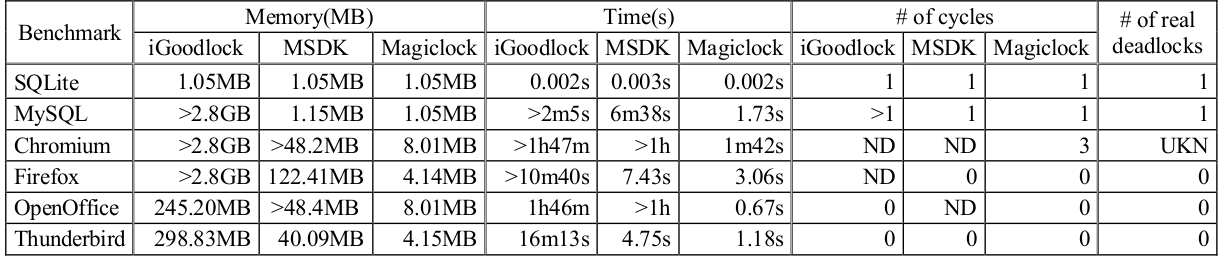
\includegraphics[width=12cm]{img/magicfuzzerbenchmark.png}
\end{table}

For some programs, the test would simple start the program and then close it when the interface appears.
Other programs used test cases adopted from bug reports in their own repositories.
The difference of test strategies was due to the inexistence of benchmarks of large-scale C/C++ programs with test cases that could repeat occurrences of deadlocks.
After evaluating the results of tests, it was concluded that MagicFuzzer could run efficiently with low memory consumption compared to similar techniques, like MulticoreSDK \cite{mcsdk}.

%\subsection{Avoiding deadlock avoidance.}%
In another study, Pyla et al. \cite{sammati}
present Sammati as a dynamic analysis tool which is capable of automatically detecting deadlocks and recovering for any threaded application that use the pthreads interface,
transparently detecting and eliminating deadlocks in threaded codes.
It is implemented as a library that overloads the standard pthreads interface and turns locks into a deadlock-free operation. Since it is just a library overload,
it does not require any modifications to application source code.

Sammati's approach makes memory updates to be only visible outside of the critical section when all parent locks are released, by associating memory accesses
with locks and specifying ownership of memory updates within a critical section to a set of locks. When a deadlock is detected, one of the threads involved in the deadlock is
chosen as a victim and rolled back to the point of acquisition of the offending lock, discarding all memory updates done.
Then it is safe to restart the code that runs into that critical section again because the memory updates never were made visible outside of the critical
section, thus providing recovery from deadlock.

Differently from transactional memory systems, it does not significantly impact performance because its runtime privatizes memory at page granularity instead of instrumenting
individual load/store operations. To implement containment for threaded codes, it was used a technique described in \cite{berger}: if each thread had its own virtual address space,
such as most recent UNIX operating systems, privatization can be implemented efficiently in a runtime environment where threads are converted to $cords$ (a single threaded process).
In Sanmati, threads were converted to cords transparently. Since all cords share a global address space, the deadlock detection algorithm has access to the holding and waiting
sets of each cord and the deadlock detection can be performed at the time a lock is acquired.

The detection algorithm uses a global hash table that associates locks being held with its owning cord, another hash table to associate a cord with a lock it is waiting on and a
queue per cord of locks acquired. The algorithm then tries to acquire some requested lock in a non-blocking attempt. When the acquisition is successful, the acquired lock is
inserted in the first hash table and into that cord's queue. However, if the acquisition fails, then the algorithm finds which cord is the owner of that lock and checks if that
cord is waiting for another lock. If this is not the case, then there's no cycle, so deadlock algorithm inserts that lock in the second hash table and finally try to attempt
the same lock in a blocking way. But if that is the case, then it moves on to check which cord is the owner of the next lock, thus transversing the waiting relationship graph
until a cycle is detected. The complexity of this detection algorithm is linear and has upper bound of $\mathcal{O}$(n).

Sanmati's evaluation analysed threaded applications such as Phoenix \cite{phoenix}, SPLASH \cite{splash} and a few synthetic benchmark suites which contain programs written
intentionally to create deadlocks. Sanmati shows a performance comparable to pthreads for most applications and in a few cases it could even perform better according to the researchers.
Memory overhead remained below 2 MB independently of the number of the cords in all programs tested.

Qin et al. \cite{rx} proposes a dynamic approach called Rx that rolls back a server application once a bug occurs to a checkpoint,
trying to modify the server environment on its re-execution. In that study, bugs are treated as "allergies" and different program executions
could either have the "allergen" or not. In the context of concurrency bugs such as deadlocks, as timing is essential for deadlocks to manifest,
a retry of the server request that caused a deadlock could be enough to get rid of the deadlock.

Rx works by dynamically changing the execution environment based on the failure symptoms, and then
executing again the same code region that contained the bug, but now in the new environment. If the re-execution successfully pass through the problematic period,
the all environment changes are disabled, so time and space overheads are avoided. By intercepting memory-related library calls such as $malloc()$, $realloc()$,
$calloc()$, $free()$, etc., a memory wrapper was implemented to provide environmental changes: during normal execution, it will simply invoke the corresponding
standard memory management library calls, which incurs little overhead. Then at re-execution phase (called $recovery$ mode), the memory wrapper would activate
a memory-related environmental change instructed by the control unit.

In evaluation experiments executed for that study, in general, Rx recovered from software failure in about 0.16 seconds, which was 21-53 times faster than the whole program restart approach they did before. Such efficiency enables servers to provide non-stop services despite software failures caused by common software defects.


\section{Hybrid analysis}

It is also possible to mix both static analysis and dynamic analysis in an hybrid analysis to take advantage of both types and boost performance.
Some techniques deploy static analysis to infer deadlock types and dynamic analysis for the parts of the program that could not be analysed in the first part,
reducing the overhead caused by dynamic analysis drastically.

%\subsection{Preventing database deadlocks in applications.}%
In Grechanik et al. study \cite{grechanik},
a novel approach known as REDACT would statically detect all hold-and-wait cycles among resources in SQL statements and prevent database deadlocks automatically: a supervisory
program that prevents database deadlocks was designed to intercept transactions sent by applications to databases dynamically. Once a potential deadlock is detected, the
conflicting transaction is delayed and the deadlock cycle is broken. It performs its static analysis at compile time to prevent deadlocks at runtime. This separation enables the algorithm to avoid expensive computations at runtime and instead it does a simple lookup in the hold-and-wait cycles already detected earlier, turning deadlock prevention fast and efficient.

However, the first step would involve some manual-effort on every application that uses a database, where all transactions used by them should be extracted.
Once the SQL statements were extracted, the static analysis phase begins and these transactions are parsed. These parsed results are used as input for a modeler that automatically transforms SQL statements into abstract operations
and synchronization requests which is used by hold-and-wait detection algorithm. Once these cycles are detected, they are used as input to a supervisory control in the dynamic analysis.

The dynamic phase is responsible to prevent database deadlocks automatically. The first step is to add interceptors in the application with callbacks associated with particular events.
Instead of sending SQL statements from application to the database, the interceptors divert the statements to the supervisory controller whose goal is to quickly analyse if
hold-and-wait cycles are present in the SQL statements that are currently in the execution queue. If no hold-and-wait cycle is present, then it forwards these statements to the
database for execution; otherwise, it holds back one SQL statement while allowing others to proceed, and once these statements are executed and results are sent back to applications,
the held back statament is finally sent to be executed by the database, thus effectively preventing the database deadlock.

Database deadlocks are typically detected within database engines at runtime, raising deadlock exceptions and rolling back transactions involved in the circular wait. Programmers
can write special handling for such situations, but most of the time they just repeat aborted operations. Thus database deadlocks may degrade performance significantly and the
effort of REDACT is to prevent them to ever happen.

However not all hold-and-wait cycles detected in the static analysis will actually lead to database deadlocks, so false positives are possible.
Some optimizations in the database may prevent it from raising an exception even in cases where a deadlock can be easily identified.
Thus it's only possible to know if there's a deadlock in the database when the statement is executed and this approach to prevent deadlocks
consequently imposes an overhead in addition to some reduction in the level of parallelism in applications.

In a performance evaluation, an extreme case scenario with a total of 5,000 SQL statements took aproximately 6.5 hours for the static analysis to finish and detect all hold-and-wait
cycles. In a more realistic case of a large scale application with more than 50 statements, all cycles were found in less than 2 seconds. However, all subject programs used in the
experimental evaluation were relatively small mostly because it is difficult to find large open-source applications that largely use non-trivial database transactions.

REDACT's cycle analysis has exponential complexity and this poses a limitation for it to deal with ultra large-scale transactions. Also, when the static analysis
produces too many false positives of hold-and-wait cycles, it may cause big performance overhead, but this evaluation was left as a proposal for future work.

\subsection{Deadlocks as Exceptions}

% TODO: move this to the proper place
In Haskell, deadlock exceptions happens when garbage collector detects a thread as unreachable \footnote{http://goo.gl/v09kqn}.
